\documentclass[10pt,a4paper]{article}
\usepackage[a4paper,outer=1cm,inner=1cm,top=3cm,bottom=3cm]{geometry}
\usepackage{gensymb}
\usepackage{graphicx}
\graphicspath{{./documents/}{./figs}}
\begin{document}
\begin{enumerate}
\item In the givien figure, PQ is tangent to the circle centred at $\vec{o}$. If \angle{AOB}=$95^{\degree}$, then the measure of \angle{ABQ} will be
\begin{figure}[!h]
\centering
	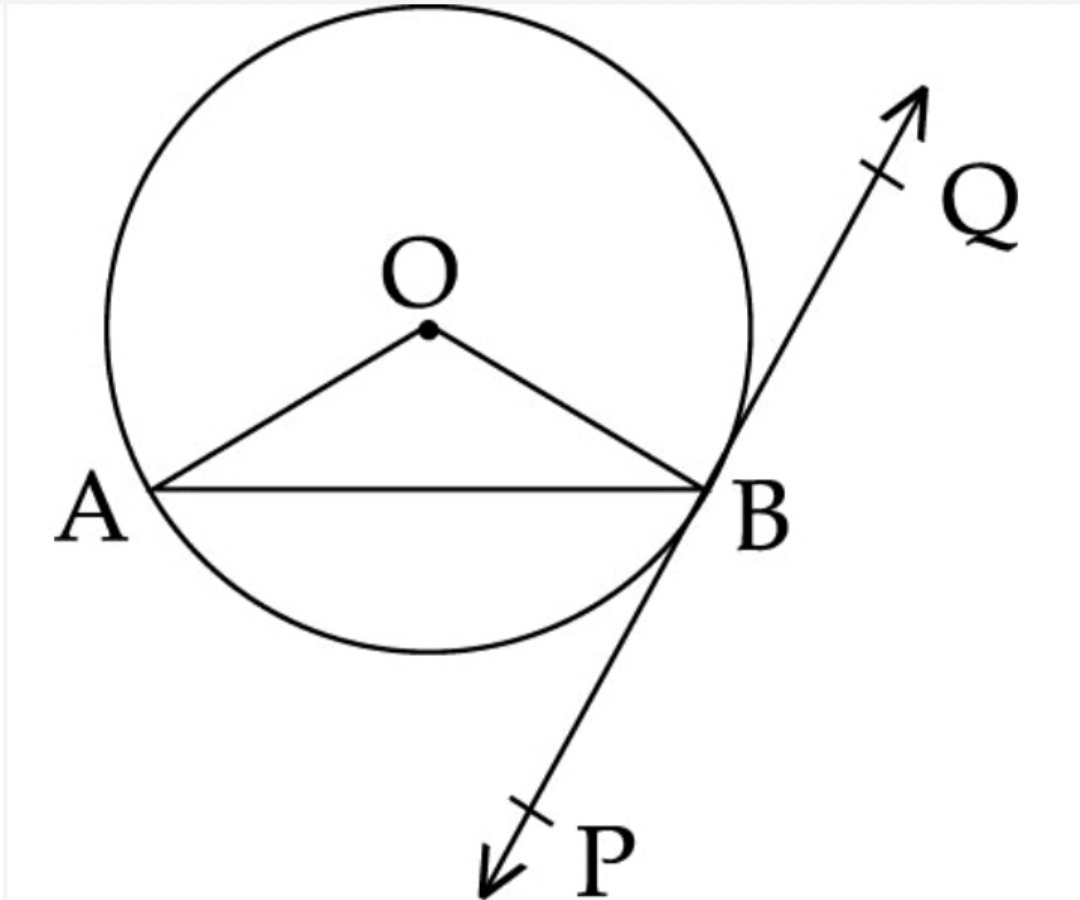
\includegraphics[scale=0.15]{fig1.jpg}
	\caption{circle1}
	\label{fig=pic}
\end{figure}
		\begin{enumerate}
			\item $47.5^{\degree}$
			\item $42.5^{\degree}$
			\item $85^{\degree}$
			\item $95^{\degree}$
		\end{enumerate}
	\item (a) Two tangents TP and TQ are drawn to a circle with center $\vec{o}$ from an external point T.
		prove that \angle{PTQ}=2\angle{OPQ}
		\begin{figure}[!h]
			\centering
			\includegraphics[scale=0.35]{fig2.jpg}
			\caption{circle2}
			\label{fig=pic}
		\end{figure}
		$$\textbf{OR}$$
		(b) In the givien figure, a circle is inscribed in a quadrilatrals ABCD in which 
		\angle{B}=$90^{\degree}$. If AD=7cm,AB=20cm and DS=3cm, then find the radius of circle
		\begin{figure}[!h]
			\centering
			\includegraphics[scale=0.12]{fig3.jpg}
			\caption{circle3}
			\label{fig=pic}
		\end{figure}
	\item The discus throw is an event in which an atlete attempts to throw a discus.the athlete spins anti-
		clockwise around one and a half times through a circle, then the throw. When released,then discus travel along the tanget to the circular spin orbit.
		\begin{figure}[!h]
			\centering
			\includegraphics[scale=0.08]{fig4.jpg}
		\end{figure}\\
		In the givien figure,AB is one such tangent to a circle of radius 75cm.Point $\vec{o}$ is center 
		of the circle and \angle{AOB}=$30^{\degree}$.PQ is parallel to OA
		\begin{figure}[!h]
			\centering
			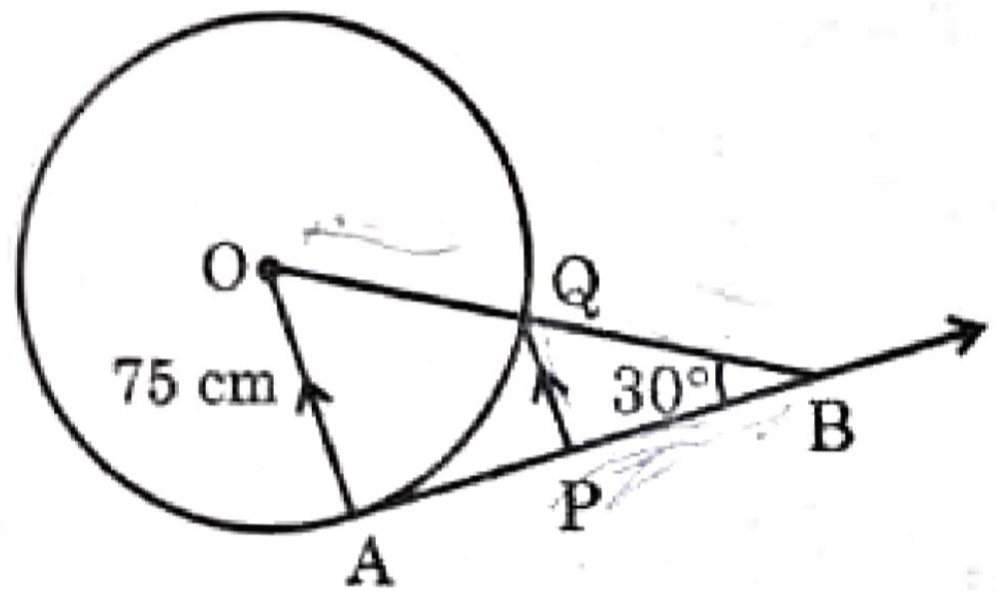
\includegraphics[scale=0.13]{fig5.jpg}
			\caption{circle5}
		        \label{fig=pic}
		\end{figure}\\
		Based on above information:
		\begin{enumerate}
			\item find the length of AB.
			\item find the length of OB.
			\item find the length of PQ.
		\end{enumerate}
	\item In the givien figure, the quadrilateral PQRS cirumscribes a circle.here PA+CS is equal to:
		\begin{figure}[!h]
			\centering
			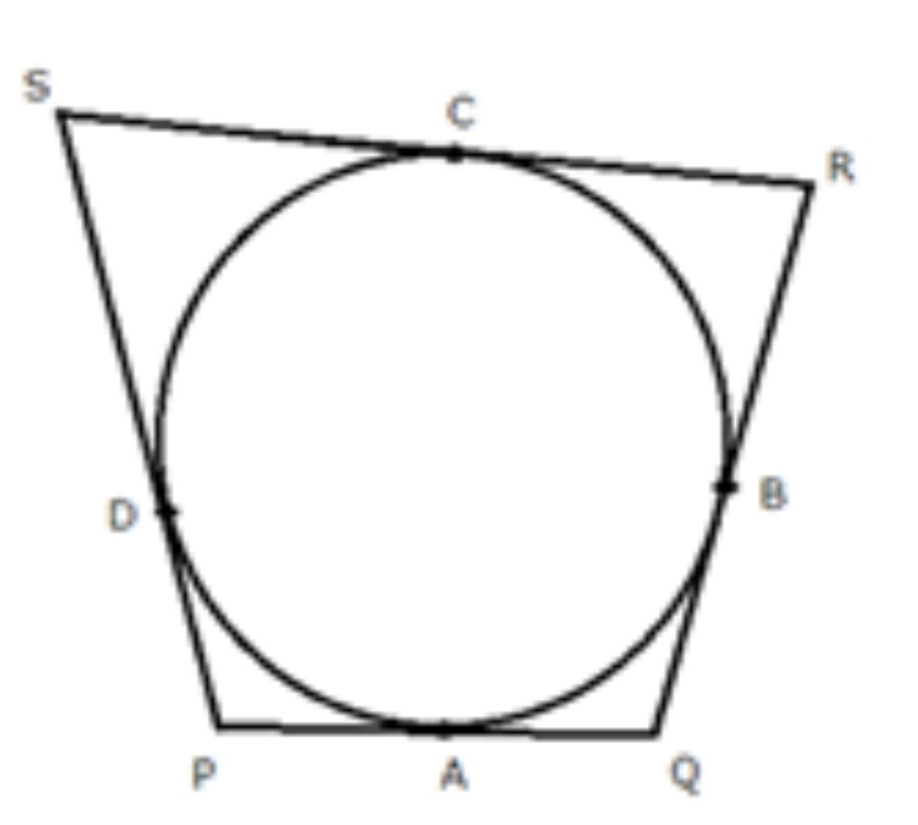
\includegraphics[scale=0.18]{fig6.jpg}
			\caption{circle6}
			\label{fig=pic}
		\end{figure}
		\begin{enumerate}
			\item QR
			\item PS
			\item PR
			\item PQ
		\end{enumerate}
	\item In the givien figure, $\vec{o}$ is the center of the circle. AB and AC are tangents drawn to the
		circle from point A.If \angle{BAC}=$65{\degree}$, then find the measure of \angle{BOC}.
		\begin{figure}[!h]
			\centering
			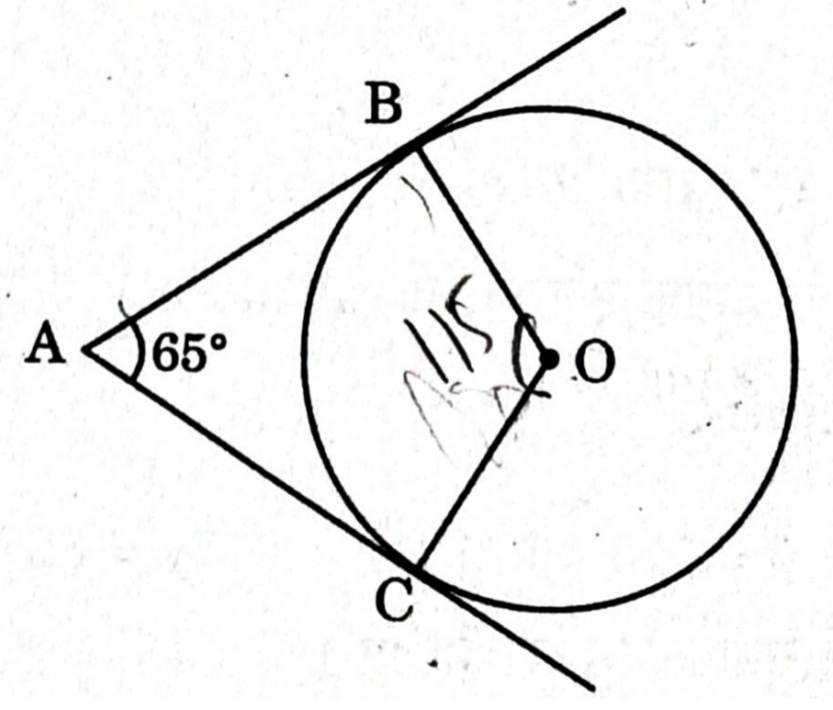
\includegraphics[scale=0.19]{fig7.jpg}
			\caption{circle7}
			\label{fig=pic}
		\end{figure}
	\item In the givien figure, $\vec{o}$ is the center of the circle and BCD is a tangent to it at p. Prove 
		that \angle{BAC}+\angle{ACD}=90$^{\degree}$\\
		\begin{figure}[h!]
              \centering          
        	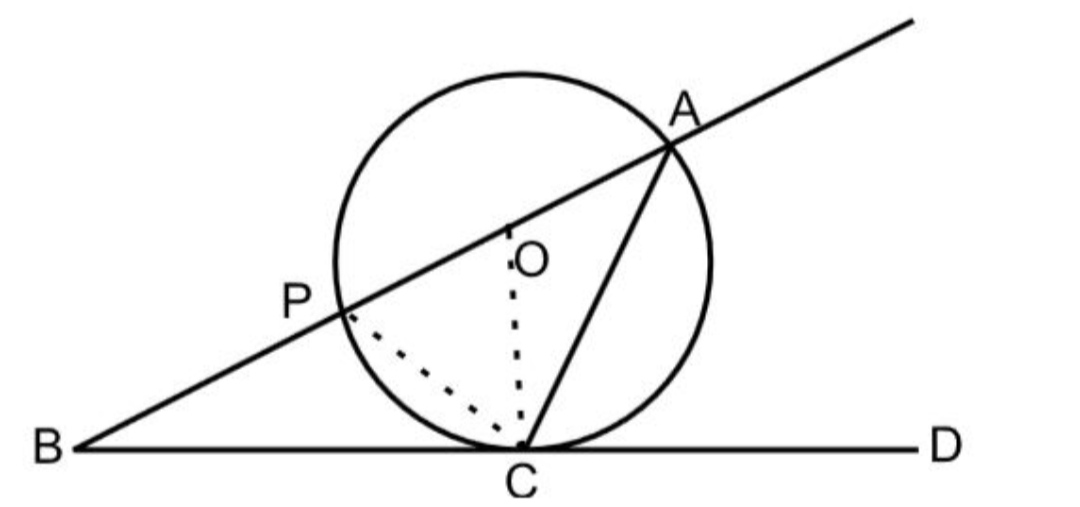
\includegraphics[scale=0.25]{fig8.jpg}     
                        \caption{circle8}  
                        \label{fig=pic}
		\end{figure}
	\item In the givien figure,PT is a tangent to the circle with center $\vec{O}$.If \angle{TPO}=
		$25^{\degree}$,then x is equal to:
		\begin{figure}[h!]
			\centering
			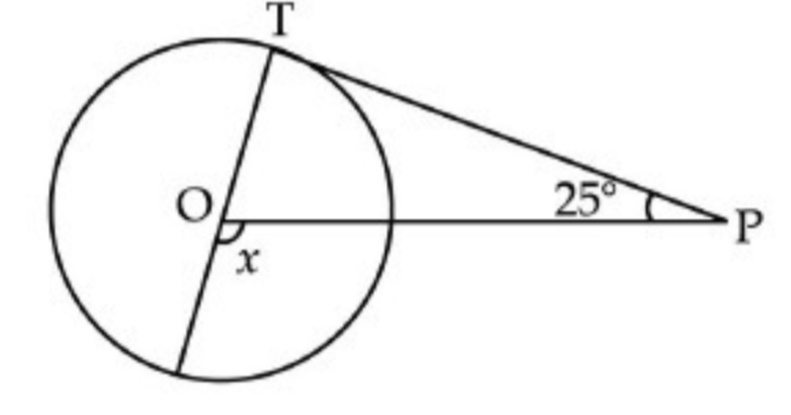
\includegraphics[scale=0.32]{fig9.jpg}
			\caption{circle9}
			\label{fig=pic}
		\end{figure}
		\begin{enumerate}
			\item $25^{\degree}$
			\item $65^{\degree}$
			\item $90^{\degree}$
			\item $115^{\degree}$
		\end{enumerate}
	\item In the givien,TA is a tangent tothe circle with center $\vec{O}$ such that OT=4cm, \angle{OTA}=$30^
		{\degree}$,then length of TA is:
		\begin{figure}[!h]
			\centering
			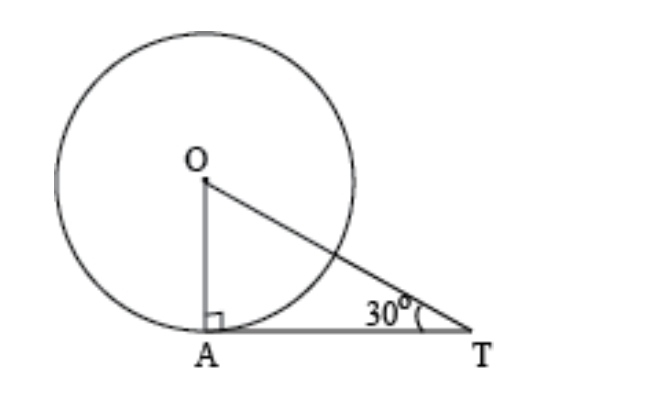
\includegraphics[scale=0.3]{fig10.jpg}
			\caption{circle10}
			\label{fig=pic}
		\end{figure}
		\begin{enumerate}
			\item 2$\sqrt{3}$cm
			\item 2cm
			\item 2$\sqrt{2}$cm
			\item $\sqrt{3}$cm
		\end{enumerate}
	\item Two concentric circles are of radii 5cm and 3cm. Find the length of he chord of the larger circle 
		which touches the smaller circle






	
\end{enumerate}
\end{document}
